\begin{figure}[t]
    \centering
    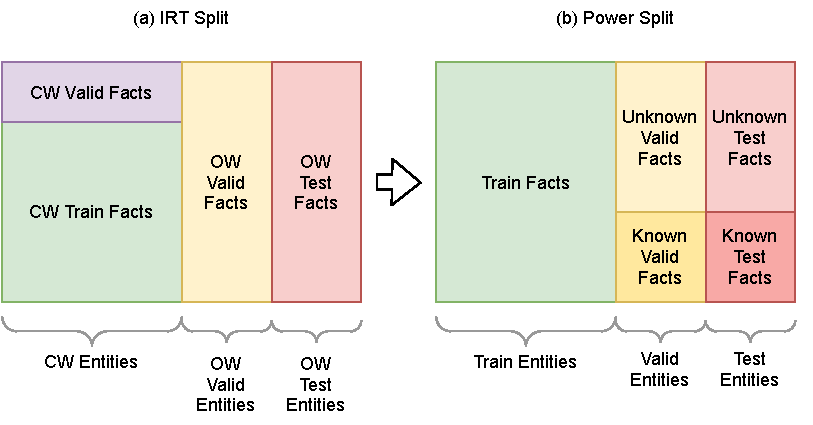
\includegraphics[width=\textwidth]{5_experiments/2_power_splits/power_split}
    \caption{Repartitioning an IRT fact split into a Power split by merging the training fact subsets and splitting open-world validation and test subsets into facts are known and unknown during inference, respectively.}
    \label{fig:5_experiments/2_power_splits/power_split}
\end{figure}

Theoretically, an IRT fact split and matching text set are sufficient for training the Power model. However, when evaluating the trained model against the IRT split's open-world entities, Power would perform only mediocre as it could only use its Texter component for inference since the open-world entities do not provide any facts the Ruler can work with. Therefore, the IRT splits are transformed to \emph{Power splits}, which divide the validation and test facts into so-called \emph{known facts} and \emph{unknown facts}. During inference, only known facts may be used to apply rules, while both known and unknown facts form the ground truth during evaluation -- neither known nor unknown validation and test facts are seen during rule mining. IRT separate closed-world training and validation facts are merged as there is no need for the latter. \autoref{fig:5_experiments/2_power_splits/power_split} illustrates the repartitioning of the IRT splits.

\begin{table}[t]
    \makebox[\textwidth][c]{
        \begin{tabular}{ l r c r r c r r }
    \toprule
    
    \multicolumn{1}{l}{\textbf{Power Split}} &
    \multicolumn{1}{c}{\textbf{Train Facts}} & \phantom &
    \multicolumn{1}{c}{\textbf{\thead{Known \\ Valid Facts}}} &
    \multicolumn{1}{c}{\textbf{\thead{Known \\ Valid Facts \\ per Entity}}} & \phantom &
    \multicolumn{1}{c}{\textbf{\thead{Known \\ Test Facts}}} &
    \multicolumn{1}{c}{\textbf{\thead{Known \\ Test Facts \\ per Entity}}} \\

    \midrule

    CDE-0   & \multirow{6}{*}{\num{137738}} && \num{0}     & \num{0.00}  && \num{0}     & \num{0.00}  \\
    CDE-5   &                               && \num{2062}  & \num{0.71}  && \num{1378}  & \num{0.73}  \\
    CDE-15  &                               && \num{6186}  & \num{2.12}  && \num{4136}  & \num{2.18}  \\
    CDE-30  &                               && \num{12372} & \num{4.24}  && \num{8273}  & \num{4.36}  \\
    CDE-50  &                               && \num{20620} & \num{7.07}  && \num{13788} & \num{7.27}  \\
    CDE-100 &                               && \num{41240} & \num{14.13} && \num{27577} & \num{14.54} \\

    \midrule

    FB-0   & \multirow{6}{*}{\num{238191}} && \num{0}     & \num{0.00}  && \num{0}     & \num{0.00} \\
    FB-5   &                               && \num{2325}  & \num{1.50}  && \num{1271}  & \num{1.56} \\
    FB-15  &                               && \num{6975}  & \num{4.51}  && \num{3813}  & \num{4.67} \\
    FB-30  &                               && \num{13950} & \num{9.03}  && \num{7626}  & \num{9.35} \\
    FB-50  &                               && \num{23251} & \num{15.05} && \num{12711} & \num{15.58} \\
    FB-100 &                               && \num{46503} & \num{30.01} && \num{25423} & \num{31.16} \\
    
    \bottomrule
\end{tabular}

    }
    \caption{Power splits with varying ratios of known validation and test fact. For example, ``CDE-50'' denotes the CoDEx-M-based Power split with half of the test facts being available for rule application during inference while the FB-0 Power split does not reveal any of the FB15k-237 facts during inference.}
    \label{tab:5_experiments/2_power_splits/power_splits_table}
\end{table}

The ratio of known and unknown facts can be varied when creating the Power split to study the Ruler's effectiveness on entities with more or less given knowledge. \autoref{tab:5_experiments/2_power_splits/power_splits_table} lists the splits used for the evaluation. For readability, the Power splits based on the CoDEx-M and FB15k-237 splits are referred to and ``CDE'' and ``FB'', respectively. An integer suffix specifies the chosen percentage of known validation and test facts. For example, the CDE-50 Power split denotes the Power split created from the IRT CoDEx-M split with 50\% of the validation and test facts being available for rule application during inference. In practice, the CDE-15 and FB-5 splits are particularly interesting, because they represent few-shot scenarios with only one or two known test facts per entity. The CDE-0 and FB-0 splits correspond to zero-shot open-world scenarios.

Along with the creation of the Power split, the question of appropriate metrics for the evaluation arises. While evaluation scenarios for classical fact splits typically consider micro precision, recall, and F1 across all facts, this work regards macro precision, recall, F1, and mAP averaged over the test entities, as this comes closer to the goal of producing top predictions for as many entities as possible -- while the micro metrics could achieve good results if the model preferred overall good predictions over entities with few ground truth facts. It should be noted, however, that not further described experiments with the micro metrics yielded similar results to the macro ones. As a ranking metric, mean average precision has been preferred over mean reciprocal rank because it does not focus on the single best prediction for an entity, which comes closer to the intended use case of suggesting multiple facts for KGC, as well. For entities for which no predictions are made, precision is mathematically undefined. In this case, the precision for that entity is set to 1 since no incorrect predictions were made. Similarly, recall and mAP are undefined when there are no ground truth facts for an entity. In these rare cases, recall and mAP are set to 1 if no predictions were made for the entity and 0 otherwise.
